\documentclass[11pt]{article}
%Gummi|065|=)
\title{\textbf{CS 361 Homework 2}}
\author{Nathaniel Murphy (njmurph3)}
\date{}

\usepackage{a4wide}
\usepackage{amsmath}
\usepackage{amsfonts}
\usepackage{graphicx}

\begin{document}

\maketitle

\section*{2.1}
\[r=0.9,\hspace{1mm}\bar{x} = 150,\hspace{1mm}\sigma_x=30,\hspace{1mm}\bar{y}=0.8,\hspace{1mm}\sigma_y=0.1\]
\subsection*{(a)}
\[\hat{x}^p=\frac{170-150}{30}=\frac{20}{30}=\frac{2}{3}\]
\[\hat{y}^p=r\hat{x}^p=0.9\Big(\frac{2}{3}\Big)=0.6\]
\[y_p=\hat{y}^p(\sigma_y)+\bar{y}=0.6(0.1)+0.8=\textbf{0.86\text{ lbs}}\]
\subsection*{(b)}
\[\hat{y}^p=\frac{0.75-0.8}{0.1}=-0.5\]
\[\hat{x}^p=r\hat{y}^p=0.9(-0.5)=-0.45\]
\[x^p=\hat{x}^p(\sigma_x)+\bar{x}=(-0.45)(30)+150=\textbf{136.5\text{ lbs}}\]
\subsection*{(c)}
We expect this prediction to be reliable because $r=0.9$, so the predict3ed normalized coordinates should fall close to the $\hat{y}=\hat{x}$ line, whereas the predicted value is $\hat{y}=r\hat{x}$.
\clearpage
\section*{2.2}
\[r=0.3,\hspace{1mm}\bar{x}=60,000,\hspace{1mm}\sigma_x=20,000,\hspace{1mm}\bar{y}=100,\hspace{1mm}\sigma_y=15\]
\subsection*{(a)}
\[\hat{x}^p=\frac{70000-60000}{20000}=0.5\]
\[\hat{y}^p=r\hat{x}^p=(0.3)(0.5)=0.15\]
\[y_p=\hat{y}^p(\sigma_y)+\bar{y}=(0.15)(15)+100=102.25\]
\subsection*{(b)}
We expect this prediction to be not very accurate, given the correlation between $x$ and $y$ to be 0.3.
\subsection*{(c)}
\[\bar{x}'=\bar{x}+c\]
\[\hat{x}^p=\frac{x^p-\bar{x}'}{\sigma_x}=\frac{x^p-(\bar{x}+c)}{\sigma_x}=\frac{x^p-\bar{x}-c}{\sigma_x}\]
\[\hat{y}^p=r\cdot\hat{x}^p=r\cdot\frac{x^p-\bar{x}-c}{\sigma_x}\]
\[\hat{y}^p=\Big(r\cdot\frac{x^p-\bar{x}-c}{\sigma_x}\Big)\sigma_y+\bar{y}\]
\[(x^p-\bar{x}-c)\frac{r\sigma_y}{\sigma_x}+\bar{y}<(x^p-\bar{x})\frac{r\sigma_y}{\sigma_x}+\bar{y}\]
\[(x^p-\bar{x}-c)\frac{r\sigma_y}{\sigma_x}<(x^p-\bar{x})\frac{r\sigma_y}{\sigma_x}\]
\[(x^p-\bar{x}-c)<(x^p-\bar{x})\]
We see that the inequality holds because $c>0$.
\clearpage
\section*{2.3}
\[\text{corr}(\{x,y\})=\frac{\Sigma_i\hat{x}_i\hat{y}_i}{N}=\frac{(\hat{x}_1\hat{y}_1+\hat{x}_2\hat{y}_2+\ldots+\hat{x}_N\hat{y}_N)}{N}=\frac{(\hat{y}_1\hat{x}_1+\hat{y}_2\hat{x}_2+\ldots+\hat{y}_N\hat{x}_N}{N}\]
\[=\frac{\Sigma_i\hat{y}_i\hat{x}_i}{N}=\text{corr}(\{y,x\})\]
We can do this by the commutative property of multiplication.
\\[20mm]
\section*{2.5}
\ \\[10mm]
\subsection*{(a)}
Assume that mean$(\{u\})=0$, $\hat{x}_i^p=a\hat{y}_i+b$, $u_i=\hat{x}_i-\hat{x}_i^p$.
\[u_i=\hat{x}_i-\hat{x}_i^p\Rightarrow\text{ mean}(\{u\})=\frac{1}{N}\Sigma_i\big(\hat{x}_i-\hat{x}_i^p\big)=\frac{1}{N}\Sigma_i\big(\hat{x}_i-a\hat{y}-b\big)=\frac{1}{N}\Sigma_i(\hat{x}_i)-\frac{1}{N}\Sigma_i(a\hat{y})-\frac{1}{N}\Sigma_i(b)\]
\[=\text{mean}(\{\hat{x}\})-a\frac{1}{N}\Sigma_i(\hat{y})-b\]
\[=\text{mean}(\{x\})-a\cdot\text{mean}(\hat{y})-b\]
\[=0-0-b\]
\[=b,\text{ and since mean}(\{x\})=0,\hspace{1mm}b\text{ must be 0}.\]
\clearpage
\subsection*{(b)}
Find $\text{min}_{a\in\mathbb{R}}$ var$(\{u\})=$ var$(\{\hat{x}_i-\hat{x}_i^p\})=$ var$(\{\hat{x}_i-a\hat{y_i}-b\})$
\[=\text{mean}(\{(\hat{x}_i-a\hat{y}_i)^2\})\]
\[=\text{mean}(\{\hat{x}_i^2-a\hat{x}_i\hat{y}_i+a^2\hat{y}_i\})\]
\[=\text{mean}(\{\hat{x}_i^2\})-\text{ mean}(\{2a\hat{x}_i\hat{y}_i\})+\text{ mean}(\{a^2\hat{y}_i^2\})\]
\[=1-2ar+a^2\]
Take the derivative with respect to $a$ to find the minimum.
\[\frac{d}{da}\Big(1-2ar+a^2\Big)=-2r+2a\]
\[-2r+2a=0\]
\[2r=2a\]
\[r=a\]
The coefficient that minimizes var$(\{u\})$ is $a=r$.
\\[20mm]
\subsection*{(c)}
Looking at figure 2.21, we can see that the closer $r$ gets to 1, the closer the lines get together (until convergence at $y=x$). While some people would say that plotting as close to the lin $y=x$ is the best choice, this directly contradicts our $r$ value if it is less than 1. In this particular example, we see that when $\hat{x}^p>0$, we might generally under predict with $\hat{y}_p$ and when $x_p<0$ we may generally overpredict. But this is also true for predicting with $\hat{y}^p$ vice versa, and it is a way that we can keep our predicted normalized data at the right distance away from the $y=x$ line.
\clearpage
\section*{2.6}
\subsection*{(a) $y_p=2014.5$}
\[\hat{y}^p=\frac{2014.5-1988.5}{14}=1.86\]
\[\hat{T}^p=r\hat{y}^p=0.892(1.86)=1.66\]
\[T^p=\hat{T}^p(\sigma_T)+\text{ mean}(\{T\})=1.66(0.231)+0.175=\textbf{0.558}\]
\subsection*{(b) $y_p=2028.5$}
\[\hat{y}^p=\frac{2028.5-1988.5}{14}=2.55\]
\[\hat{T}^p=r\hat{y}^p=0.892(2.86)=2.55\]
\[T^p=\hat{T}^p(\sigma_T)+\text{ mean}(\{T\})=2.55(0.231)+0.175=\textbf{0.764}\]
\subsection*{(c) $y_p=2042.5$}
\[\hat{y}^p=\frac{2042.5-1988.5}{14}=3.86\]
\[\hat{T}^p=r\hat{y}^p=0.892(3.86)=3.44\]
\[T^p=\hat{T}^p(\sigma_T)+\text{ mean}(\{T\})=3.44(0.231)+0.175=\textbf{0.970}\]
\clearpage
\section*{2.7}
\subsection*{(a) $T^p=0.5$}
\[\hat{T}^p=\frac{0.5-0.175}{0.231}=1.41\]
\[\hat{n}_t^p=r\hat{T}^p=0.471(1.41)=0.664\]
\[n_t^p=\hat{n}_t^p(\sigma_{n_t}+\text{ mean}(\{n_t\})=0.664(30.8)+31.6=\textbf{52.1}\]
\subsection*{(b) $T^p=0.6$}
\[\hat{T}^p=\frac{0.6-0.175}{0.231}=1.84\]
\[\hat{n}_t^p=r\hat{T}^p=0.471(1.84)=0.867\]
\[n_t^p=\hat{n}_t^p(\sigma_{n_t}+\text{ mean}(\{n_t\})=0.867(30.8)+31.6=\textbf{58.3}\]
\subsection*{(c) $T^p=0.7$}
\[\hat{T}^p=\frac{0.7-0.175}{0.231}=2.27\]
\[\hat{n}_t^p=r\hat{T}^p=0.471(2.27)=1.07\]
\[n_t^p=\hat{n}_t^p(\sigma_{n_t}+\text{ mean}(\{n_t\})=1.07(30.8)+31.6=\textbf{64.6}\]
\clearpage
\section*{2.8}
\subsection*{(a)}
\begin{figure}[h!]
	\centering
	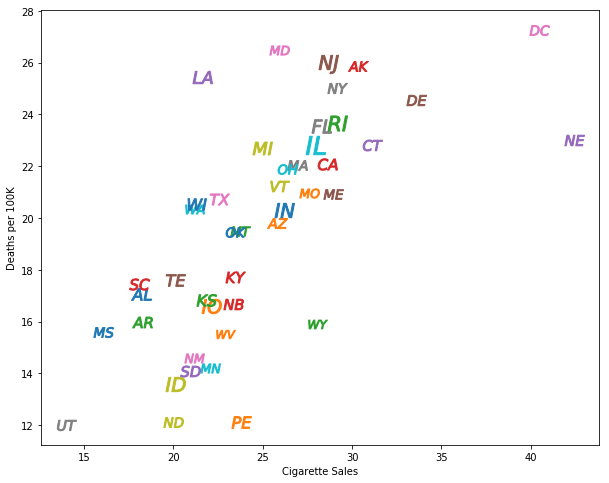
\includegraphics[width=100mm]{lung_cig.png}
	\caption{We see that the two outliers are Nevada and Washington D.C.}
\end{figure}
\begin{figure}[h!]
	\centering
	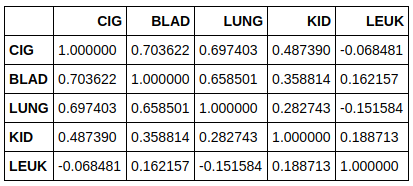
\includegraphics[width=80mm]{with_outliers_corr.png}
	\caption{Correlations for data with outliers}
\end{figure}
\begin{figure}[h!]
	\centering
	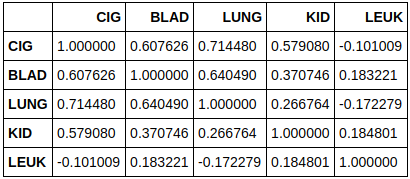
\includegraphics[width=80mm]{wo_outliers_corr.png}
	\caption{Correlations for data without outliers}
\end{figure}
\clearpage
\subsection*{(b)}
We can see that the correlation between per capita cigarette sales and lung cancer deaths per 100K population with the outliers is $r=0.6974$ and without the outliers is $r=0.7145$. Taking out the outliers raised our correclation coefficient because it has been proven that smoking cigarettes increases the risk of lung cancer in individuals. With the commuting and tourism factors taken out, we could see those people that bought cigarettes and died within the same state.
\subsection*{(c)}
We can see that the correlation between per capita cigarette sales and bladder cancer deaths per 100K population with the outliers is $r=0.7036$ and without the outliers is $r=0.6076$. This phenomenon is not very explainable in the sense that smoking is a risk factor in contracting bladder cancer, however, upon further examination, the survival rates by stage of bladder cancer are relatively higher than lung cancer. Thus, more people being treated implies that less people die from bladder cancer.
\subsection*{(d)}
We can see that the correlation between per capita cigarette sales and kidney cancer deaths per 100K population with the outliers is $r=0.4874$ and without the outliers is $r=0.5791$. Research has shown that smokers have an increased risk of kidney cancer than non-smokers. We see that the correlation is still relatively low with respect to the other cancers, which might be due to the fact that the main cause of kidney cancer is a family history.
\subsection*{(e)}
We can see that the correlation between per capita cigarette sales and leukemia deaths per 100K population with the outliers is $r=-0.0685$ and without the outliers is $r=-0.101$. We see that there is little to no negative correlation between cigarette sales and leukemia. Removing the outliers doesn't change this, so we still see a very low correlation.
\subsection*{(f)}
Even though we have computed a positive correlation between cigarette sales and lung cancer deaths, we cannot state that smoking causes lung cancer because we are merely exmanining correlation, which is completely different than causation.
\subsection*{(g)}
As with the previous question, any correlation that we examine cannot be interpreted as causation. Even further, the correlation that we did observe was extremely low so we expect no relationship between cigarette sales and leukemia.
\end{document}
